\documentclass[12pt]{article}
\usepackage{fullpage}
\usepackage{setspace}
\usepackage{upquote}
\usepackage{tikz}
\usepackage{graphicx}
\usepackage{listings}
\title{CS411 Team Fructose - Final Report for Minecraft Inventory Bank}
\author{Steven Biersteker, Grace Chow, Aaron Gallant, Jason Sze}
\date{UIUC Spring 2011}

\lstset{language=SQL}
\lstset{upquote=true} % sensible quotes
\lstset{showstringspaces=false} % no special string spaces


\begin{document}

\maketitle

\section{What we accomplished}
Our team created a Minecraft plugin and web application platform allowing for easier manipulation of large quantities of materials within the game. It supports players using simple commands to quickly store and recover large quantities of items. It also has a webpage interface that allows users to check their inventory and compare with others, searching to see who has the most items or money in general or who holds a specific item.

\section{Why is our project useful?}
Minecraft is an extremely popular ($>$1.9 million copies sold\footnote{http://www.minecraft.net/stats.jsp}) ``sandbox'' style game, where the fun comes from how the player chooses to explore and build. Materials can be used to craft a variety of items or stacked to build almost anything imaginable. Players have already created many elaborate constructions, ranging from world monuments to re-imaginings of other videogames\footnote{http://www.geekosystem.com/21-amazing-minecraft-creations/}. These epic creations require a lot of time and in-game materials, and our project makes it much easier for players to get started with their massive Minecraft constructions.

Without our plugin, materials are purely manipulated with gameplay mechanics. This means that players must manually harvest, transport, and store (in game-built chests) any materials they may wish to stockpile for a large project. Using our plugin it is now possible for players to simply type commands to quickly store and retrieve their materials, as well as buy and trade with other users. Game balance is still preserved via a leaderboard and economy that allows users to be aware and sure they are paying a fair price for resources, and all information is easily accessible from a web application so users don't need to start Minecraft to check their information.

\section{Data/database}
Our database is powered by MySQL, and designed as follows.

\subsection{ER Diagram and Schema}
The ER diagram is shown in figure 1. Represented in our MySQL database, the schema is shown in figure 2. Our schema, in relational algebra, has the following three tables:

\begin{itemize}
  \item User(user\_id, name, password\_hash)
  \item Inventory(user\_id, item\_id, quantity)
  \item Item(item\_id, name, metadata, block\_id)
\end{itemize}

\begin{figure}[h]
  \centerline{% Graphic for TeX using PGF
% Title: /home/aaron/Documents/CS/i2cs/cs411/project1/er1.dia
% Creator: Dia v0.97.1
% CreationDate: Sun Apr 17 15:13:29 2011
% For: aaron
% \usepackage{tikz}
% The following commands are not supported in PSTricks at present
% We define them conditionally, so when they are implemented,
% this pgf file will use them.
\ifx\du\undefined
  \newlength{\du}
\fi
\setlength{\du}{15\unitlength}
\begin{tikzpicture}
\pgftransformxscale{1.000000}
\pgftransformyscale{-1.000000}
\definecolor{dialinecolor}{rgb}{0.000000, 0.000000, 0.000000}
\pgfsetstrokecolor{dialinecolor}
\definecolor{dialinecolor}{rgb}{1.000000, 1.000000, 1.000000}
\pgfsetfillcolor{dialinecolor}
\definecolor{dialinecolor}{rgb}{1.000000, 1.000000, 1.000000}
\pgfsetfillcolor{dialinecolor}
\fill (5.050000\du,5.000000\du)--(5.050000\du,6.800000\du)--(7.990000\du,6.800000\du)--(7.990000\du,5.000000\du)--cycle;
\pgfsetlinewidth{0.100000\du}
\pgfsetdash{}{0pt}
\pgfsetmiterjoin
\definecolor{dialinecolor}{rgb}{0.000000, 0.000000, 0.000000}
\pgfsetstrokecolor{dialinecolor}
\draw (5.050000\du,5.000000\du)--(5.050000\du,6.800000\du)--(7.990000\du,6.800000\du)--(7.990000\du,5.000000\du)--cycle;
% setfont left to latex
\definecolor{dialinecolor}{rgb}{0.000000, 0.000000, 0.000000}
\pgfsetstrokecolor{dialinecolor}
\node at (6.520000\du,6.100000\du){User};
\definecolor{dialinecolor}{rgb}{1.000000, 1.000000, 1.000000}
\pgfsetfillcolor{dialinecolor}
\fill (20.300000\du,4.950000\du)--(20.300000\du,6.750000\du)--(23.240000\du,6.750000\du)--(23.240000\du,4.950000\du)--cycle;
\pgfsetlinewidth{0.100000\du}
\pgfsetdash{}{0pt}
\pgfsetmiterjoin
\definecolor{dialinecolor}{rgb}{0.000000, 0.000000, 0.000000}
\pgfsetstrokecolor{dialinecolor}
\draw (20.300000\du,4.950000\du)--(20.300000\du,6.750000\du)--(23.240000\du,6.750000\du)--(23.240000\du,4.950000\du)--cycle;
% setfont left to latex
\definecolor{dialinecolor}{rgb}{0.000000, 0.000000, 0.000000}
\pgfsetstrokecolor{dialinecolor}
\node at (21.770000\du,6.050000\du){Item};
\definecolor{dialinecolor}{rgb}{1.000000, 1.000000, 1.000000}
\pgfsetfillcolor{dialinecolor}
\fill (12.850000\du,5.796500\du)--(14.427500\du,4.850000\du)--(16.005000\du,5.796500\du)--(14.427500\du,6.743000\du)--cycle;
\pgfsetlinewidth{0.100000\du}
\pgfsetdash{}{0pt}
\pgfsetmiterjoin
\definecolor{dialinecolor}{rgb}{0.000000, 0.000000, 0.000000}
\pgfsetstrokecolor{dialinecolor}
\draw (12.850000\du,5.796500\du)--(14.427500\du,4.850000\du)--(16.005000\du,5.796500\du)--(14.427500\du,6.743000\du)--cycle;
% setfont left to latex
\definecolor{dialinecolor}{rgb}{0.000000, 0.000000, 0.000000}
\pgfsetstrokecolor{dialinecolor}
\node[anchor=east] at (12.550000\du,5.496500\du){};
\definecolor{dialinecolor}{rgb}{0.000000, 0.000000, 0.000000}
\pgfsetstrokecolor{dialinecolor}
\node[anchor=west] at (16.305000\du,5.496500\du){};
\definecolor{dialinecolor}{rgb}{0.000000, 0.000000, 0.000000}
\pgfsetstrokecolor{dialinecolor}
\node at (14.427500\du,5.996500\du){Has};
\pgfsetlinewidth{0.100000\du}
\pgfsetdash{}{0pt}
\pgfsetdash{}{0pt}
\pgfsetbuttcap
{
\definecolor{dialinecolor}{rgb}{0.000000, 0.000000, 0.000000}
\pgfsetfillcolor{dialinecolor}
% was here!!!
\definecolor{dialinecolor}{rgb}{0.000000, 0.000000, 0.000000}
\pgfsetstrokecolor{dialinecolor}
\draw (7.990000\du,5.900000\du)--(12.850000\du,5.796500\du);
}
\pgfsetlinewidth{0.100000\du}
\pgfsetdash{}{0pt}
\pgfsetdash{}{0pt}
\pgfsetbuttcap
{
\definecolor{dialinecolor}{rgb}{0.000000, 0.000000, 0.000000}
\pgfsetfillcolor{dialinecolor}
% was here!!!
\definecolor{dialinecolor}{rgb}{0.000000, 0.000000, 0.000000}
\pgfsetstrokecolor{dialinecolor}
\draw (16.005000\du,5.796500\du)--(20.300000\du,5.850000\du);
}
\definecolor{dialinecolor}{rgb}{1.000000, 1.000000, 1.000000}
\pgfsetfillcolor{dialinecolor}
\pgfpathellipse{\pgfpoint{14.490000\du}{9.700000\du}}{\pgfpoint{2.540000\du}{0\du}}{\pgfpoint{0\du}{0.900000\du}}
\pgfusepath{fill}
\pgfsetlinewidth{0.100000\du}
\pgfsetdash{}{0pt}
\definecolor{dialinecolor}{rgb}{0.000000, 0.000000, 0.000000}
\pgfsetstrokecolor{dialinecolor}
\pgfpathellipse{\pgfpoint{14.490000\du}{9.700000\du}}{\pgfpoint{2.540000\du}{0\du}}{\pgfpoint{0\du}{0.900000\du}}
\pgfusepath{stroke}
% setfont left to latex
\definecolor{dialinecolor}{rgb}{0.000000, 0.000000, 0.000000}
\pgfsetstrokecolor{dialinecolor}
\node at (14.490000\du,9.900000\du){quantity};
\pgfsetlinewidth{0.100000\du}
\pgfsetdash{}{0pt}
\pgfsetdash{}{0pt}
\pgfsetbuttcap
{
\definecolor{dialinecolor}{rgb}{0.000000, 0.000000, 0.000000}
\pgfsetfillcolor{dialinecolor}
% was here!!!
\definecolor{dialinecolor}{rgb}{0.000000, 0.000000, 0.000000}
\pgfsetstrokecolor{dialinecolor}
\draw (14.427500\du,6.743000\du)--(14.490000\du,8.800000\du);
}
\definecolor{dialinecolor}{rgb}{1.000000, 1.000000, 1.000000}
\pgfsetfillcolor{dialinecolor}
\pgfpathellipse{\pgfpoint{7.647500\du}{1.950000\du}}{\pgfpoint{2.347500\du}{0\du}}{\pgfpoint{0\du}{0.900000\du}}
\pgfusepath{fill}
\pgfsetlinewidth{0.100000\du}
\pgfsetdash{}{0pt}
\definecolor{dialinecolor}{rgb}{0.000000, 0.000000, 0.000000}
\pgfsetstrokecolor{dialinecolor}
\pgfpathellipse{\pgfpoint{7.647500\du}{1.950000\du}}{\pgfpoint{2.347500\du}{0\du}}{\pgfpoint{0\du}{0.900000\du}}
\pgfusepath{stroke}
% setfont left to latex
\definecolor{dialinecolor}{rgb}{0.000000, 0.000000, 0.000000}
\pgfsetstrokecolor{dialinecolor}
\node at (7.647500\du,2.150000\du){user\_id};
\pgfsetdash{}{0pt}
\definecolor{dialinecolor}{rgb}{0.000000, 0.000000, 0.000000}
\pgfsetstrokecolor{dialinecolor}
\draw (6.300000\du,2.350000\du)--(8.995000\du,2.350000\du);
\definecolor{dialinecolor}{rgb}{1.000000, 1.000000, 1.000000}
\pgfsetfillcolor{dialinecolor}
\pgfpathellipse{\pgfpoint{2.320000\du}{3.100000\du}}{\pgfpoint{1.770000\du}{0\du}}{\pgfpoint{0\du}{0.900000\du}}
\pgfusepath{fill}
\pgfsetlinewidth{0.100000\du}
\pgfsetdash{}{0pt}
\definecolor{dialinecolor}{rgb}{0.000000, 0.000000, 0.000000}
\pgfsetstrokecolor{dialinecolor}
\pgfpathellipse{\pgfpoint{2.320000\du}{3.100000\du}}{\pgfpoint{1.770000\du}{0\du}}{\pgfpoint{0\du}{0.900000\du}}
\pgfusepath{stroke}
% setfont left to latex
\definecolor{dialinecolor}{rgb}{0.000000, 0.000000, 0.000000}
\pgfsetstrokecolor{dialinecolor}
\node at (2.320000\du,3.300000\du){name};
\definecolor{dialinecolor}{rgb}{1.000000, 1.000000, 1.000000}
\pgfsetfillcolor{dialinecolor}
\pgfpathellipse{\pgfpoint{4.352500\du}{8.950000\du}}{\pgfpoint{3.502500\du}{0\du}}{\pgfpoint{0\du}{0.900000\du}}
\pgfusepath{fill}
\pgfsetlinewidth{0.100000\du}
\pgfsetdash{}{0pt}
\definecolor{dialinecolor}{rgb}{0.000000, 0.000000, 0.000000}
\pgfsetstrokecolor{dialinecolor}
\pgfpathellipse{\pgfpoint{4.352500\du}{8.950000\du}}{\pgfpoint{3.502500\du}{0\du}}{\pgfpoint{0\du}{0.900000\du}}
\pgfusepath{stroke}
% setfont left to latex
\definecolor{dialinecolor}{rgb}{0.000000, 0.000000, 0.000000}
\pgfsetstrokecolor{dialinecolor}
\node at (4.352500\du,9.150000\du){password\_hash};
\pgfsetlinewidth{0.100000\du}
\pgfsetdash{}{0pt}
\pgfsetdash{}{0pt}
\pgfsetbuttcap
{
\definecolor{dialinecolor}{rgb}{0.000000, 0.000000, 0.000000}
\pgfsetfillcolor{dialinecolor}
% was here!!!
\definecolor{dialinecolor}{rgb}{0.000000, 0.000000, 0.000000}
\pgfsetstrokecolor{dialinecolor}
\draw (4.352500\du,8.050000\du)--(5.050000\du,6.800000\du);
}
\pgfsetlinewidth{0.100000\du}
\pgfsetdash{}{0pt}
\pgfsetdash{}{0pt}
\pgfsetbuttcap
{
\definecolor{dialinecolor}{rgb}{0.000000, 0.000000, 0.000000}
\pgfsetfillcolor{dialinecolor}
% was here!!!
\definecolor{dialinecolor}{rgb}{0.000000, 0.000000, 0.000000}
\pgfsetstrokecolor{dialinecolor}
\draw (2.320000\du,4.000000\du)--(5.050000\du,5.000000\du);
}
\pgfsetlinewidth{0.100000\du}
\pgfsetdash{}{0pt}
\pgfsetdash{}{0pt}
\pgfsetbuttcap
{
\definecolor{dialinecolor}{rgb}{0.000000, 0.000000, 0.000000}
\pgfsetfillcolor{dialinecolor}
% was here!!!
\definecolor{dialinecolor}{rgb}{0.000000, 0.000000, 0.000000}
\pgfsetstrokecolor{dialinecolor}
\draw (7.647500\du,2.850000\du)--(6.520000\du,5.000000\du);
}
\definecolor{dialinecolor}{rgb}{1.000000, 1.000000, 1.000000}
\pgfsetfillcolor{dialinecolor}
\pgfpathellipse{\pgfpoint{20.047500\du}{1.650000\du}}{\pgfpoint{2.347500\du}{0\du}}{\pgfpoint{0\du}{0.900000\du}}
\pgfusepath{fill}
\pgfsetlinewidth{0.100000\du}
\pgfsetdash{}{0pt}
\definecolor{dialinecolor}{rgb}{0.000000, 0.000000, 0.000000}
\pgfsetstrokecolor{dialinecolor}
\pgfpathellipse{\pgfpoint{20.047500\du}{1.650000\du}}{\pgfpoint{2.347500\du}{0\du}}{\pgfpoint{0\du}{0.900000\du}}
\pgfusepath{stroke}
% setfont left to latex
\definecolor{dialinecolor}{rgb}{0.000000, 0.000000, 0.000000}
\pgfsetstrokecolor{dialinecolor}
\node at (20.047500\du,1.850000\du){item\_id};
\pgfsetdash{}{0pt}
\definecolor{dialinecolor}{rgb}{0.000000, 0.000000, 0.000000}
\pgfsetstrokecolor{dialinecolor}
\draw (18.700000\du,2.050000\du)--(21.395000\du,2.050000\du);
\definecolor{dialinecolor}{rgb}{1.000000, 1.000000, 1.000000}
\pgfsetfillcolor{dialinecolor}
\pgfpathellipse{\pgfpoint{25.720000\du}{2.650000\du}}{\pgfpoint{1.770000\du}{0\du}}{\pgfpoint{0\du}{0.900000\du}}
\pgfusepath{fill}
\pgfsetlinewidth{0.100000\du}
\pgfsetdash{}{0pt}
\definecolor{dialinecolor}{rgb}{0.000000, 0.000000, 0.000000}
\pgfsetstrokecolor{dialinecolor}
\pgfpathellipse{\pgfpoint{25.720000\du}{2.650000\du}}{\pgfpoint{1.770000\du}{0\du}}{\pgfpoint{0\du}{0.900000\du}}
\pgfusepath{stroke}
% setfont left to latex
\definecolor{dialinecolor}{rgb}{0.000000, 0.000000, 0.000000}
\pgfsetstrokecolor{dialinecolor}
\node at (25.720000\du,2.850000\du){name};
\definecolor{dialinecolor}{rgb}{1.000000, 1.000000, 1.000000}
\pgfsetfillcolor{dialinecolor}
\pgfpathellipse{\pgfpoint{27.090000\du}{5.550000\du}}{\pgfpoint{2.540000\du}{0\du}}{\pgfpoint{0\du}{0.900000\du}}
\pgfusepath{fill}
\pgfsetlinewidth{0.100000\du}
\pgfsetdash{}{0pt}
\definecolor{dialinecolor}{rgb}{0.000000, 0.000000, 0.000000}
\pgfsetstrokecolor{dialinecolor}
\pgfpathellipse{\pgfpoint{27.090000\du}{5.550000\du}}{\pgfpoint{2.540000\du}{0\du}}{\pgfpoint{0\du}{0.900000\du}}
\pgfusepath{stroke}
% setfont left to latex
\definecolor{dialinecolor}{rgb}{0.000000, 0.000000, 0.000000}
\pgfsetstrokecolor{dialinecolor}
\node at (27.090000\du,5.750000\du){metadata};
\definecolor{dialinecolor}{rgb}{1.000000, 1.000000, 1.000000}
\pgfsetfillcolor{dialinecolor}
\pgfpathellipse{\pgfpoint{24.340000\du}{9.150000\du}}{\pgfpoint{2.540000\du}{0\du}}{\pgfpoint{0\du}{0.900000\du}}
\pgfusepath{fill}
\pgfsetlinewidth{0.100000\du}
\pgfsetdash{}{0pt}
\definecolor{dialinecolor}{rgb}{0.000000, 0.000000, 0.000000}
\pgfsetstrokecolor{dialinecolor}
\pgfpathellipse{\pgfpoint{24.340000\du}{9.150000\du}}{\pgfpoint{2.540000\du}{0\du}}{\pgfpoint{0\du}{0.900000\du}}
\pgfusepath{stroke}
% setfont left to latex
\definecolor{dialinecolor}{rgb}{0.000000, 0.000000, 0.000000}
\pgfsetstrokecolor{dialinecolor}
\node at (24.340000\du,9.350000\du){block\_id};
\pgfsetlinewidth{0.100000\du}
\pgfsetdash{}{0pt}
\pgfsetdash{}{0pt}
\pgfsetbuttcap
{
\definecolor{dialinecolor}{rgb}{0.000000, 0.000000, 0.000000}
\pgfsetfillcolor{dialinecolor}
% was here!!!
\definecolor{dialinecolor}{rgb}{0.000000, 0.000000, 0.000000}
\pgfsetstrokecolor{dialinecolor}
\draw (24.340000\du,8.250000\du)--(23.240000\du,6.750000\du);
}
\pgfsetlinewidth{0.100000\du}
\pgfsetdash{}{0pt}
\pgfsetdash{}{0pt}
\pgfsetbuttcap
{
\definecolor{dialinecolor}{rgb}{0.000000, 0.000000, 0.000000}
\pgfsetfillcolor{dialinecolor}
% was here!!!
\definecolor{dialinecolor}{rgb}{0.000000, 0.000000, 0.000000}
\pgfsetstrokecolor{dialinecolor}
\draw (24.550000\du,5.550000\du)--(23.240000\du,5.850000\du);
}
\pgfsetlinewidth{0.100000\du}
\pgfsetdash{}{0pt}
\pgfsetdash{}{0pt}
\pgfsetbuttcap
{
\definecolor{dialinecolor}{rgb}{0.000000, 0.000000, 0.000000}
\pgfsetfillcolor{dialinecolor}
% was here!!!
\definecolor{dialinecolor}{rgb}{0.000000, 0.000000, 0.000000}
\pgfsetstrokecolor{dialinecolor}
\draw (24.468400\du,3.286400\du)--(23.240000\du,4.950000\du);
}
\pgfsetlinewidth{0.100000\du}
\pgfsetdash{}{0pt}
\pgfsetdash{}{0pt}
\pgfsetbuttcap
{
\definecolor{dialinecolor}{rgb}{0.000000, 0.000000, 0.000000}
\pgfsetfillcolor{dialinecolor}
% was here!!!
\definecolor{dialinecolor}{rgb}{0.000000, 0.000000, 0.000000}
\pgfsetstrokecolor{dialinecolor}
\draw (20.047500\du,2.550000\du)--(21.770000\du,4.950000\du);
}
\pgfsetlinewidth{0.100000\du}
\pgfsetdash{}{0pt}
\pgfsetdash{}{0pt}
\pgfsetbuttcap
{
\definecolor{dialinecolor}{rgb}{0.000000, 0.000000, 0.000000}
\pgfsetfillcolor{dialinecolor}
% was here!!!
\definecolor{dialinecolor}{rgb}{0.000000, 0.000000, 0.000000}
\pgfsetstrokecolor{dialinecolor}
\draw (27.090000\du,5.550000\du)--(27.090000\du,5.550000\du);
}
\end{tikzpicture}
}
  \caption{ER Diagram}
\end{figure}

\begin{figure}[h]
  \centerline{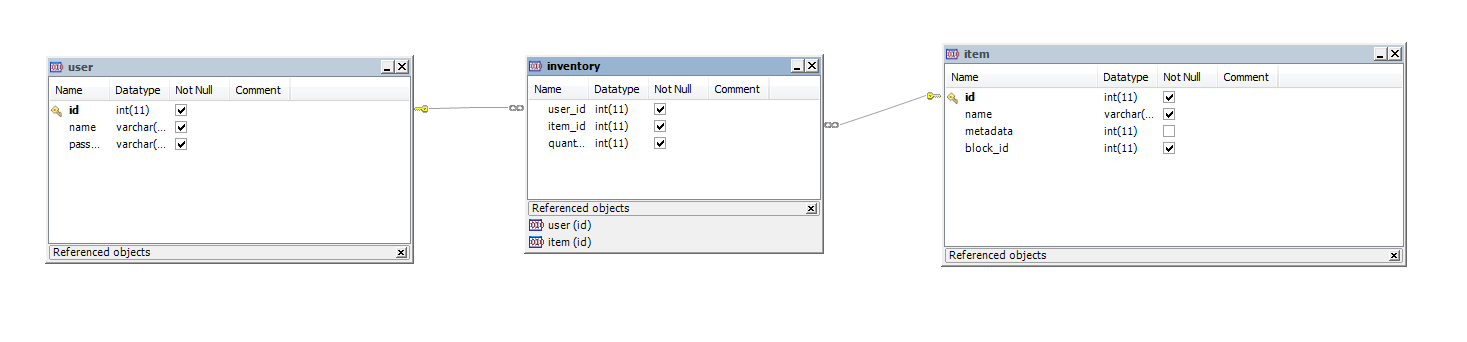
\includegraphics[width=22cm]{db.png}}
  \caption{MySQL Database Schema}
\end{figure}

\subsection{Data sources}
Our data comes from plugin usage. When installed on a Minecraft server, any users who login will have the option of storing or retrieving materials in their inventory with this plugin. At present the plugin is running on a server used by UIUC Minecraft players\footnote{http://mother.dyndns.tv/inventorybank/}, but we intend to share our plugin so that other Minecraft servers and players around the world can enjoy it (and the code is already freely available on a GitHub repository\footnote{https://github.com/Kazooie/Minecraft-Inventory-Bank}).

\section{Project functionality}
\begin{itemize}
  \item Basic Functions: Insert/update/delete: Text commands for storing/retrieving items
  \begin{itemize}
    \item Create user for website use, log in to website
    \item Graphical view of items on the website
    \item Search: Look up inventory by user
  \end{itemize}
  \item Advanced Functions: Implement shop and trading sections on the website
  \begin{itemize}
    \item Create a basic economy trading system with supply and demand calculations
    \item Set up kit creation: sets of items that players can load/unload
    \item Offer pages to rank players by money, items
  \end{itemize}
\end{itemize}

\section{Basic function example}
Following is the query and process by which we generate the leaderboard in terms of inventory size (amount of materials stored). The query returns a ranked list of users and their inventory size, and this data is then displayed within our web application.

\subsection{SQL used}
  \begin{lstlisting}
    SELECT u.name AS username, SUM(i.quantity) AS inventory_size
    FROM user u, inventory i
    WHERE u.id = i.user_id
    GROUP BY 1
    ORDER BY 2 DESC;
  \end{lstlisting}

\subsection{Dataflow steps}
First the actual data is initially inserted into the database via usage of the plugin from Minecraft. The plugin, and Minecraft itself, are written in Java, and use the MySQL Java Connector to insert and update records. The web application is written in PHP, and uses the built in PHP MySQL functionality to run the query and return the results. These results are displayed to the user with a combination of HTML and CSS for formatting.

\section{Advanced functions}
Our advanced functionality centers around allowing users to quickly buy the materials they need to craft certain items or build other creations.

\subsection{In-game shop functionality}
In addition to storing items, the Inventory Bank can act as a storefront. Users are able to list materials for sale or buy materials from others, with prices set relatively according to supply and demand. This is important because it is possible for a user to find an oversupply of one valuable resource (e.g. diamonds) but not enough of another (e.g. gold). They can sell the resources they no longer want and buy those that they do. This can also allow users with large reserves but lacking a particular common material (e.g. wood) to simply buy large quantities rather than go to the trouble of harvesting it for themselves.

This is done via similar text commands to material storage and retrieval. ADD EXAMPLES.

\subsection{Kit creation}
Many interesting Minecraft creations have specific recipes, listing different quantities of different raw materials needed to craft an item. Kits allow a user to quickly retrieve the exact needed materials for a specific item from their inventory bank. ADD EXAMPLES, OR SWITCH.

\section{Technical challenges}
Some story, preferably about something simple like a db connection hiccup.

\section{How well we lined up with our plan}


\section{Final division of labor}
\begin{itemize}
  \item Steven Biersteker - Minecraft plugin, server/db administration, ...
  \item Grace Chow - Webapp design (inventory management), styling (CSS), ...
  \item Aaron Gallant - Minecraft plugin (soon I swear!), final report, ...
  \item Jason Sze - Webapp design (user login), PHP/MySQL communication, ...
\end{itemize}


\end{document}
